\documentclass[11pt]{article}

\usepackage[margin=1in,footskip=0.25in]{geometry}

%\usepackage{helvet}
%\renewcommand{\familydefault}{\sfdefault}

\renewcommand\refname{\vskip -1cm}

%\renewcommand{\rmdefault}{phv} % Arial
%\renewcommand{\sfdefault}{phv} % Arial
\usepackage{setspace}
\usepackage{wrapfig}
\usepackage{amsmath}
\usepackage{amssymb}
\usepackage{graphicx}
\usepackage{mathrsfs}
\usepackage{bm}
\usepackage{wasysym}
\usepackage{placeins}
\usepackage{multirow}
\usepackage[T1]{fontenc}
\usepackage[super]{natbib}
\usepackage{framed}
\usepackage{caption}
\usepackage{longtable}

\begin{document}

\title{Tissue isotope dynamics}

\maketitle

\section{Methods}

\subsection{Isotopic dynamics of a resource specialist}

We start by considering a set of prey items, each with its own range $\delta^{13}C$ and $\delta^{15}N$ values, which we (for now) assume are independent and normally distributed.
We then consider a consumer that selects among these prey items and integrates the isotopic values of prey into its tissues.
The integration of the isotopic values of a prey item is thus a weighted average of the consumer's isotopic values and the isotopic values of the prey, with respect to the different mass of each.

For simplicity, we will assume that a single prey item is consumed over the course of a day.
Even though prey individuals are of different sizes, we will assume that the biomass of consumed prey is the same over the course of each day (i.e. that the consumer is replacing the energy that it spends). 
If $X_c$ is the isotopic value of the consumer, and $X_p$ is the isotopic value of a prey, then

\begin{align}
	X_c(t+1) &= \frac{M_c}{M_c + M_p}X_c(t) + \frac{M_p}{M_c + M_p}X_p(t) \\ \nonumber
	&= fX_c(t) + (1-f)X_p(t)
\end{align}

\noindent where $f$ is the proportion of total biomass that is the consumer's body tissues at the end of the day (i.e. minus body mass spent via metabolism).
The change over time is then

\begin{align}
\label{diffeq}
	X_c(t+1) - X_c(t) &= fX_c(t) + (1-f)X_p(t) - X_c(t),~~\mbox{equivalent to} \\
	\frac{\rm d}{\rm dt}X_c &= fX_c + (1-f)X_p - X_c,
\end{align}

\noindent in continuous time. 
The above differential equation describes how the consumer's biomass changes as it incorporates the mass of some prey $p$.
Note that - for now - we are assuming that the consumer is specializing on a single prey.
Solving for Eq. \ref{diffeq} reveals a tissue incorporation decay curve $X_c = X_p + (X_0-X_p)\exp\{(f-1)t\}$, where a tissue starts with an isotope value $X_0$ and at the limit $t\rightarrow \infty $, we find that $X_c \rightarrow X_p$, which means that the consumer's isotope value eventually approaches that of its only prey... it had better!

This is the exciting part! So far, we have assumed that the prey isotope value is constant, though we know that prey isotope values have variability.
We want to incorporate this idea that prey isotope values are variable, and then solve for the mean (expectation) and variability of the consumer as it eats its prey.
Just a reminder: the consumer is still a specialist, consuming a single, but variable prey.

So in this next section, we assume that $X_p \sim {\rm Norm}(\bar{x}_p,\sigma^2)$, meaning the $X_p$ is a random variable normally distributed about a mean value $\bar{x}_p$ with variance $\sigma^2$.
Then, we have to rewrite Eq. \ref{diffeq} as a Stochastic Differential Equation, which is badass

\begin{equation}
	{\rm dX_c} = fX_c{\rm dt} + (1-f)(\bar{x}_p{\rm dt} + \sigma{\rm dW}) - X_c{\rm dt}
\end{equation}

\noindent where everything is as before, except that we have this funky term to the right of $(1-f)$, which basically says that the prey isotope value varies over time (as different individuals of the same prey are consumed), and that this variability scales with $\sigma$, which is the standard deviation of the prey's isotope value, while ${\rm dW}$ is the increment of Brownian motion.

We can then solve for the expectation and variability of the consumer's isotope value (${\rm E}\{X_c\}$ and ${\rm Var}\{X_c\}$, respectively).
We find that

\begin{align}
	{\rm E}\{X_c\} &= \bar{x}_p + (X_0-\bar{x}_p){\rm e}^{(f-1)t} \nonumber \\ \nonumber \\ 
	{\rm Var}\{X_c\} &= \frac{\sigma^2(f-1)}{2}({\rm e}^{2(f-1)t} -1).
\end{align}

\noindent As before, in the limit of $t \rightarrow \infty$, ${\rm E}\{X_c\} \rightarrow \bar{x}_p$, such that the specialist consumer will be centered around its prey.
The most interesting result is that as $t \rightarrow \infty$, ${\rm Var}\{X_c\} \rightarrow \sigma^2(1-f)/2$.
Because $0 < f \leq 1$, this means that the variance of the consumer will always be less than the variance of the prey ($\sigma^2$).
The degree to which the consumer's variance is less than the prey's variance is due primarily to $f$, which describes the proportional difference between the mass of the consumer vs. the ingested resource.

\subsection{Isotopic dynamics of a prey-switching consumer}


{\bf Injecting more reality} 

Time: Seth pointed out that it would be nice to have real time units.
I think that this dynamic equation is general enough that time is just a scalar, and we can easily fix $f$ to reflect different consumption rates of prey.
For the simulations represented in the figures, I'm assuming that a sea otter weighs 20 kg at the end of the day, and that 1 kg of prey is consumed per day... so the `steady state' body mass is 21 kg.
These can be easily changed to reflect different scenarios.

Different tissues: In the above examples, we were mainly exploring how variance changed with time, and what the limit of variance would be.
The next step is to think about how different tissues accrue variability over different slices of time.
One interesting observation is that variance asymptotes really quickly.
This might be similar variability in liver vs. bone wouldn't be surprising, but needs to be explored further.
I think the tools above will be a flexible skeleton with which we can investigate the more interesting questions (such as tissues-specific variability), which are the real aim of the project.

Prey-switching: The above dynamics only apply to specialist consumers. I'm toying around with ways of generalizing foraging dynamics... I don't yet have a feel as to whether the above analyses will blow up or not when we include this, but it's in progress!

{\bf Thoughts, comments, suggestions, edits, questions?}


\begin{figure*}[h!]
   \centering
   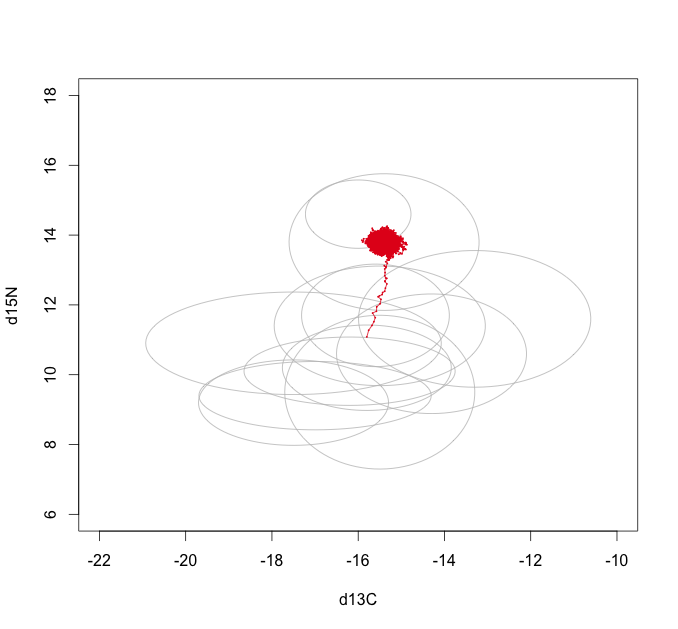
\includegraphics[width=0.5\textwidth]{fig_bivariate.png}
      \caption{
      A consumer (red) incorporating the isotopic values of a single prey species. The starting isotopic values are at the centroid of the prey space. The variability of the consumer is notably smaller than that of its prey.
      }
      \label{fig_bivariate}
\end{figure*}

\begin{figure*}[h!]
   \centering
   \includegraphics[width=0.5\textwidth]{fig_d13CvsTime.png}
      \caption{
      A) The $\delta^{13}{\rm C}$ values of the simulated consumer over time (gray points). The analytical approximation is the black line.
      B) Variability of $\delta^{13}{\rm C}$ values for the simulated forager over time. Bins are set to 200 steps; the smaller the bin, the less accurate the measure of SD.The analytical approximation for variability is the black line.
      }
      \label{fig_time}
\end{figure*}

\begin{figure*}[h!]
   \centering
   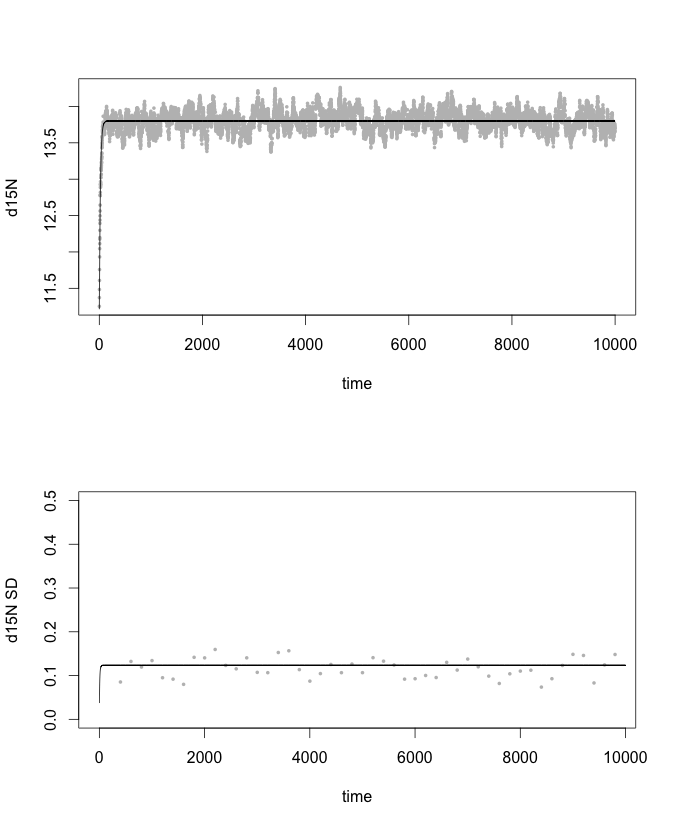
\includegraphics[width=0.5\textwidth]{fig_d15NvsTime.png}
      \caption{
      A) The $\delta^{15}{\rm N}$ values of the simulated consumer over time (gray points). The analytical approximation is the black line.
      B) Variability of $\delta^{15}{\rm N}$ values for the simulated forager over time. Bins are set to 200 steps; the smaller the bin, the less accurate the measure of SD. The analytical approximation for variability is the black line.
      }
      \label{fig_time}
\end{figure*}






\end{document}
